\documentclass[12pt, bibliography=totoc]{scrartcl}
\usepackage[headsepline,automark]{scrlayer-scrpage} %Trennlinie an Kopfzeile
%\usepackage{scrheadings}
\clearpairofpagestyles
\lohead{\rightmark}
%\renewcommand{\partmark}[1]{\relax}% \part daran hindern, den Kolumnentitel zu löschen
\ohead[]{\pagemark}
%\ofoot*{\pagemark}
%%Kopfzeile
\usepackage{txfonts} %für times new roman
%\usepackage{helvet} %für arial, dann aber 11pt
\usepackage[a4paper, left=2cm, right=2.5cm]{geometry}
\usepackage[onehalfspacing]{setspace}
%\usepackage{apacite}
\usepackage{wasysym}
\usepackage{mbenotes}
\usepackage{rotating}
%\usepackage{amsmath}
%\usepackage{amssymb}
\usepackage{float}
%\usepackage{caption}
\usepackage[T1]{fontenc}
\usepackage[utf8]{inputenc}
%\usepackage{todonotes}
\usepackage{enumitem}
%\uespackage{caption}
%\usepackage[bf]{caption}
%\renewcommand{\captionfont}{\small\slshape}
%\renewcommand{\figurename}{Abb.}
%\renewcommand{\thefigure}{\arabic{section}.\arabic{figure}}
%\makeatletter \@addtoreset{figure}{section} \makeatother
%\captionsetup[figure]{skip=1pt}
\usepackage{tabularx}
\usepackage{pdfpages}
\usepackage{array}
\usepackage{hyperref}
\usepackage{threeparttable} %fußnoten unterhalb tabelle
\usepackage{booktabs} % fuer schone Tabellen
\usepackage{rotating} % um tabellen auf quer drehen zu koennen http://www.golatex.de/kann-man-tabellen-im-querformat-darstellen-t2003.html
%\newcolumntype{C}[1]{>{\centering\arraybackslash}p{#1}} %Spalten mit fester breite zentriert
%\newcolumntype{L}[1]{>{\raggedright\arraybackslash}p{#1}} %Spalten mit fester breite linksbündig
%\newcolumntype{Y}{>{\small\raggedright\arraybackslash}X}
%\newcolumntype{C}{>{\small\centering\arraybackslash}X}
\usepackage{graphicx}
%\usepackage[german]{babel}
\usepackage{typearea}
%für Randbemerkungen, sehr nützlich:
\usepackage{xargs}                      % Use more than one optional parameter in a new commands
\usepackage[pdftex,dvipsnames]{xcolor}
\usepackage[colorinlistoftodos,prependcaption,textsize=tiny]{todonotes}
\newcommandx{\unsure}[2][1=]{\todo[linecolor=red,backgroundcolor=red!25,bordercolor=red,#1]{#2}}
\newcommandx{\change}[2][1=]{\todo[linecolor=blue,backgroundcolor=blue!25,bordercolor=blue,#1]{#2}}
\newcommandx{\info}[2][1=]{\todo[linecolor=OliveGreen,backgroundcolor=OliveGreen!25,bordercolor=OliveGreen,#1]{#2}}
\newcommandx{\improvement}[2][1=]{\todo[linecolor=Plum,backgroundcolor=Plum!25,bordercolor=Plum,#1]{#2}}
\newcommandx{\thiswillnotshow}[2][1=]{\todo[disable,#1]{#2}}
% erklaerung siehe hier http://tex.stackexchange.com/questions/9796/how-to-add-todo-notes

%hat prima funktioniert:
\usepackage[style=apa,backend=biber]{biblatex}
\usepackage[american,ngerman]{babel}
\DeclareLanguageMapping{ngerman}{ngerman-apa}
\usepackage[babel,german=guillemets]{csquotes}
%\bibliographystyle{apacite}
%nach part fängt section wieder mit eins an alte Gestaltung
%\makeatletter
%\@addtoreset{section}{part}
%\makeatother
%\renewcommand*{\partformat}{\thepart}{}
%\renewcommand*{\partheadmidvskip}{\nobreak\enskip}
%\bibliography{/Users/iNge/Dropbox/Biblio/ingesbibneu}
\bibliography{/Users/iNge/Dropbox/Biblio/library}
%\bibliography{library}




\begin{document}
\renewcommand\finalandcomma{\addcomma}

\begin{titlepage}
\thispagestyle{empty}
\begin{center}
\color{blue}\Large{Fernuniversität Hagen}\\
\end{center}


\begin{center}
\Large{Bildung und Medien: eEducation}
\end{center}
\begin{verbatim}



\end{verbatim}
\begin{center}
\textbf{\Large{Kommentierte Bibliographie zum Thema Online-Lernen}}
\end{center}
\begin{verbatim}

\end{verbatim}
\begin{center}
\textbf{Fakultät Kulturwissenschaften}
\end{center}
\begin{verbatim}










\end{verbatim}

\begin{flushleft}
\begin{tabular}{lll}
\textbf{Studiengang:} & & MA Bildung und Medien: eEducation\\
& & Modul 2: Anwendungsbezogene Bildungsforschung\\
& & \\
& & \\
\textbf{eingereicht von:} & & {\color{magenta} Inge Koch-Meinass \flq{}ingekoch@mac.com\frq{}}\\
& & {\color{magenta}Matrikelnr.: 123456 }\\
& & \\
\textbf{eingereicht am:} & & 06. November 2015\\
& & \\
& & \\
%\textbf{Betreuer:} & & Herr Prof. Dr. J. A. Müller
\end{tabular}
\end{flushleft}

% das ist wohl jetzt das Ende des Dokumentes
\end{titlepage}


%% das Papierformat zuerst
%\documentclass[a4paper, 11pt]{article}

% deutsche Silbentrennung
%\usepackage[ngerman]{babel}
%\usepackage{color} \color{blue}
% wegen deutschen Umlauten
%\usepackage[utf8]{inputenc}

% hier beginnt das Dokument
%\begin{document}

\begin{titlepage}
\thispagestyle{empty}
\begin{center}
\color{blue}\Large{Fernuniversität Hagen}\\
\end{center}


\begin{center}
%\Large{Bildung und Medien: eEducation}
\end{center}
\begin{verbatim}



\end{verbatim}
\begin{center}
\textbf{\Large{Kommentierte Bibliographie zum Thema Online-Lernen}}
\end{center}
\begin{verbatim}

\end{verbatim}
\begin{center}
%\textbf{im Studiengang Wirtschaftsinformatik}
\end{center}
\begin{verbatim}











\end{verbatim}

\begin{flushleft}
\begin{tabular}{lll}
\textbf{Studiengang:} & & MA Bildung und Medien: eEducation\\
& & Modul 2: Anwendungsbezogene Bildungsforschung\\
& & \\
& & \\
\textbf{eingereicht von:} & & {\color{magenta} Inge Koch-Meinass \flq{}ingekoch@mac.com\frq{}}\\
& & {\color{magenta}Matrikelnr.: 9650962 }\\
& & \\
\textbf{eingereicht am:} & & 06. November 2015\\
& & \\
& & \\
%\textbf{Betreuer:} & & Herr Prof. Dr. J. A. Müller
\end{tabular}
\end{flushleft}

% das ist wohl jetzt das Ende des Dokumentes
\end{titlepage}

\listoftodos[Gesammelte Unklarheiten]
\tableofcontents
%\listoftables
\setcounter{page}{1}
%\thispagestyle{empty}
\pagebreak

\section{Einleitung}\label{einleitung}

\improvement{Pisa abschneiden machte es erforderlich usw. Hier Holzkamp konkret}
\glqq Das weltweit verfügbare Wissen verdoppelt sich zurzeit alle vier
bis fünf Jahre. Der amerikanische Soziologe Richard Sennet (1998)
erwartet, dass ein ameikanischer College Student in seinem Berufsleben
elf Mal die Stelle wechselt und dreimal die Basis seines Wissens
komplett austauscht \parencite[138]{Ehlers2002}.\grqq{} Vor diesem
Hintergrund kommt der beruflichen Weiterbildung eine immer größere
Bedeutung zu, den beruflichen Anforderung gerecht zu werden, erfordert
die Bereitschaft zu lebenslangem Lernen. Mit dem Zuwachs an Veränderung
in Organisationen und der damit verbundenen Anforderung \enquote{am Ball
zu bleiben} gilt es Lernkonzepte zu finden die modernen
konstruktivistischen Lerntheorien einerseits und beruflichem Lernen von
Erwachsenen andererseits gerecht werden. Das immer größere Lernpensum,
kann nicht ausschließlich in Präsenzveranstaltung gelehrt werden,
sondern viel mehr gilt es von Zeit und Ort unabhängige Lernmöglichkeiten
zu schaffen. Digitale Lernplattformen leisten hier einen wichtigen
Beitrag und können je nach didaktischer Aufbereitung,
selbstorganisiertes, konstruktuvistisches und damit nachhaltiges Lernen
fördern.

Die vorliegende Arbeit befasst sich mit der Evaluation einer beruflichen
Weiterbildung, die als Blended Learning Kurs für FrühpädagogInnen
\footnote{Der Begriffe FrühpädagogInnen, schließt alle im Kitabereich tätigen Fachkräfte ein}
konzipiert wurde. Inhalt der Weiterbildung ist das kennenlernen und
umsetzen können des Early-Excellence Konzept, ein Ansatz mit dem
Bildungs- und Orientierungspläne der Bundesländer in den
Kindertagesstätten konzeptionell verankert werden können. Mit Hilfe
eines standardisierten Fragebogens wird versucht, den durch die
Weiterbildung gewonnen, selbsteingeschätzten Zuwachs an
Handlungskompetenz zu bestimmen. Es wird einmal das
Weiterbildungsangebot insgesamt und zum anderen der Einfluss der
digitalen Lernplattform betrachtet.

\section{Theorierahmen}\label{theorierahmen}

Der der Untersuchung zugrundeliegende Theorierahmen umfasst die Themen
Erwachsenenbildung im Blended Learning Verfahren und daraus
resultierender Zuwachs an Handlungskompetenz.

\subsection{Erwachsenenbildung}\label{erwachsenenbildung}

Das Lernen Erwachsener unterliegt besonderen Gegebenheiten, die hier
nachfolgenden beschrieben werden. Lernen im Erwachsenenalter ist
überwiegend gekennzeichnet durch Anschlusslernen. Der Erwachsene knüpft
beim Lernen an Bekanntes an, Lernen erfolgt konstruktivistisch und
subjektorientiert: „Erwachsene lassen sich in der Regel nicht belehren
oder aufklären, Wahrheiten lassen sich nicht linear vermitteln.
Erwachsene haben ihren eigenen Kopf, machen sich ihre eigenen
Gedanken\ldots`` \parencite[15]{Siebert201408}. Dies unterstreicht
einmal mehr, dass Lernen nicht hergestellt, sondern nur vom Individuum
selbst vollbracht werden kann \parencite{Faulstich2012}.

In subjektorientierten Lerntheorien z.B.: \parencite{Holzkamp2004} wird
Lernen beschrieben als eine Erweiterung von Handlungsfähigkeit und nicht
als Anhäufung von Wissen. Holzkamp prägte den Begriff des „expansiven
Lernens'', der ausdrücken soll, dass „intentionales, d.h. absichtliches
und geplantes Lernen nur dann zustande kommt, wenn das Lernsubjekt
selbst entsprechende Gründe dafür hat`` {[}\ldots{]}
\parencite[29]{Holzkamp2004}. Nach Holzkamp kommt es dann zum Lernen,
wenn das „Subjekt in seinem normalen Handlungsvollzug auf Hindernisse
oder Widerstände gestoßen ist{[}\ldots{]}.`` Im vorliegenden Fall ist
das „Hindernis`` die Einführung von Bildungs- und Orientierungsplänen in
Kitas, die es erforderlich machen den „normalen Handlungsvollzug`` zu
verändern. Diese Problematik kann nicht mit dem vorhandenen Wissen und
den vorhandenen Fähigkeiten gelöst werden, sondern erfordert das
„Einschalten einer Lernschleife`` \parencite[29]{Holzkamp2004}. Diese
Lernschleife wird mit der hier beschriebenen Weiterbildungsmaßnahme
unter Berücksichtigung, dass es unmöglich ist, Inhalte passiv in Köpfe
füllen zu können \parencite[12]{Faulstich2012}, gedreht. Schon 1993
verweist Holzkamp in seinem Buch Lernen auf die Notwendigkeit den Lerner
in den Mittelpunkt zu stellen, verweist auf den Lehr-Lern-Kurzschluss
und übt scharfe Kritik am vorherrschenden Schulsystem. Während die
didakische Umsetzung der Subjektorientierung in Schulen wenig
aufgegriffen wird, ist sie in der beruflichen Erwachsenenbildung eher
gängig \parencite{grotluschen2005expansives}.
\textcite[138]{ehlers2011qualitat} beschreibt vier Gründe für den immer
größer werdenden Stellenwert des Lerners in Weiterbildungsmaßnahemn:
\emph{Ökonomische} Gründe liegen vor, weil die Lerner Weiterbildung oft
selbst finanzieren und/oder die Weiterbildung in der Freizeit machen.
\emph{Pädagogisch-didaktische} Gründe liegen im Wandel zu
konstruktivistischen Lerntheorien, die eine Subjektorientierung
bedingen. \emph{Gesellschaftlich} ist die Entwicklung hin zur
Wissensgesellschaft zu betrachten und die Entwicklung hin zum
\emph{eLearning} als Lernform, dass per se den Lerner als Akteur
einbezieht. Auch die hier beschriebene Weiterbildungsmaßnahem orientiert
sich an den Grundlagen des subjektorientierten Lernens und vor dem
Hintergrund, dass die Teilnehmer sehr individuelle Lernzugänge haben und
letzlich nur selbst ihre Handlungsfähigkeit erweitern können. Die
Inhalte bestehen weniger in Vermittlung von Faktenwissen als vielmehr in
der Anknüpfung von bereits Erlebten in Form von Biographiearbeit und der
Berücksichtigung der jeweils unterschliedelichen Kontextbezügen. Dies
wird in den Präsenzphasen, als auch mit der Lernplattform beispielsweise
dadurch umgesetzt, dass die Lerner zugleich auch Lehrende sind, Inhalte
aktiv mitgestalten und widerum der Gemeinschaft zur Verfügung stellen.

Vor diesem Hintergrund wird in der vorliegenden Arbeit der „Lernerfolg``
eben als solche Erweiterung von Handlungsfähigkeit, in Form von Zuwachs
an Handlungskompetenz gemessen.

\subsection{Blended Learning}\label{blended-learning}

Im folgenden soll der Begriff des Blended Learning und was im Rahmen
dieser Arbeit darunter zu verstehen erläutert werden. Direkt übersetzt
bedeutet Blended Lerning „vermischtes Lernen``. Das heißt es handelt
sich bei dieser Lernform um ein Lehr-Lernsetting, dass sowohl
klassisches Face-to-Face-Lernen, als auch eLearning beinhaltet. Die
verschiedenen Lernangebote stehen sich nicht als entweder oder
gegenüber, sondern als sich ergänzend.
\texcite[3]{kerres2001multimediale} betont „dass die besondere Qualität
und auch Effizienz eines Lernangebotes vor allem in der Kombination von
Elementen unterschiedlicher methodischer und medialer Aufbereitung zum
Tragen kommt``. \textcite[45]{ehlers2011qualitat} merkt kritsch an, dass
der Begriff nicht vermischtes Lernen meint, sondern, dass es um eine
Mischung von Methoden mit denen gelernt wird, geht. „Blended Learning
strebt die Optimierung von Lernprozessen zur Erreichung individueller
Lernziele unter der Nutzung aller dafür geeigneter Lehr-Lernmethoden
an`` \parencite[46]{ehlers2011qualitat}. Blended Learning Konzepte gibt
es schon seit vielen Jahren und sie werden sowohl in Schulen und
Hochschulen , als auch in beruflichen Weiterbildungsmaßnahmen
eingesetzt. Elearning Angebote wurden in Deutschland nur sehr zögerlich
angenommen, es überwiegen in weiten Bereichen noch traditionelle
Lernformen. Aus dieser Situation heraus bot sich das Blended Learning
als Lernform an, da es traditonelle und moderne, digitale Lernformen
miteinander verbindet \parencite{Maihack2015}. Für den Einsatz von
Blended Learning sprechen nach \textcite{thomas2000evaluating}
zahlreiche Gründe: * Orts- und Zeitunabhängigkeit

\begin{itemize}
\item
  Leichte Aktualisierbarkeit
\item
  Lerner haben viel Kontrolle: sie können wählen, was sie wann lernen,
  können auf bereits durchgenommenes Material zugreifen usw.
\item
  Viele Möglichkeiten der Interaktion
\item
  Es können beliebig viele Personen am Kurs teilnehmen
\end{itemize}

Die Form des hybriden Lernens erlaubt es, Vorteile von digitalem Lernen
(selbstorganisiert, zeit- und ortsunabhängig, ) und Vorteile von
traditionellem Lernen (sich kennen lernen, Gruppen bilden, Motivation
\ldots) zu kombinieren \parencite{Zumbach2010}. Für die Gestaltung eines
eLearning Angebotes auf der Grundlage einer konstruktivistischen
Lerntheorie, ist es notwendig den Lernenden die Möglichkeit der
Eigentätigkeit, Formen des sozialen Austausches, Möglichkeiten zur
Bearbeitung komplexer Probleme usw. einzuräumen
\change{woher ist das? Zitat}. Letzlich soll dieses Lernarrangement
selbstorganisiertes und reflexives Lernen ermöglichen.

Es sei angemerkt, dass es sowohl verschiedene Begriffe, als auch
verschiedene Definitionen von Blended Learning gibt. Neben Begriffen wie
integrated Learning, flexible Learning usw. wird es im deutschen
Sprachraum oft auch als \enquote{Hybrid Teaching} benannt
\parencite{Oliver2005}\{kerres2001multimediale\}. In der vorliegenden
Arbeit meint Blended Learning, die sich ergänzende Kombination von
verschiedenen Medien, nämlich Präsenzlernen in Form von Wochendseminaren
und eLearning in Form einer Moodle-Lernplattform.

\subsection{Handlungskompetenz}\label{handlungskompetenz}

Die Qualität der hier beschriebenen Weiterbildung wird auf der Ebene des
Ergebnisses evaluiert. Wird wie oben beschreiben der Lerner in den
Mittelpunkt gerückt, kann der Lernerfolg nur der Zuwachs an
Handlungskompetenz sein. \parencite[4]{Ehlers2002}. Gemessen werden
nicht Leistungsresultate, sondern vielmehr die Fähigkeit bzw.
Disposition neue, kreative Lösungen hervorzubringen, die Messung des
Kompetenzzuwachses orientiert sich am Einzelnen und entspricht somit der
Subjektzentrierung des vorgestellten Lernarrangements
\parencite{ErpenbeckRosenstiel200305}. Handlungskompetenz meint hier die
„Fähigkeit in einer komplexen Welt gestaltend mit der Umwelt agieren zu
können`` \parencite[4]{Ehlers2002}.

Die Handlungskompetenz setzt sich nach
\textcite{ErpenbeckRosenstiel200305} aus verschiedenen Kompetenzen
zusammen, die nach \textcite{ErpenbeckRosenstiel200305} und
\autocite{Braun2008} wie folgt zusammengefasst und beschrieben werden
können:

\begin{enumerate}
\def\labelenumi{\arabic{enumi}.}
\item
  Personale Kompetenzen: Diese Kompetenz beschreibt z.B.: die Fähigkeit
  selbstorganisiert zu handeln, sich selbst einschätzen zu können,
  Motive und Werte des Handelns.
\item
  Fachkompetenz: Beschreibt Kentnisse, Verständnis,
  Anwendungsfähigkeiten und Analysefähigkeiten der Lernenden.
\item
  Methodenkompetenz: Beherrschung von Arbeitstechniken,
  Planungsvermögen, Vermögen Wissen sinnorientiert einsetzen zu können
\end{enumerate}

\% Hier dann alles zum Thema Operationalisierung

\subsection{Inhalte der Weiterbildung}\label{inhalte-der-weiterbildung}

\subsection{Aufbau der Lernplattform}\label{aufbau-der-lernplattform}

\section{Methoden}\label{methoden}

\subsection{Forschungsfrage und
Hypothesen}\label{forschungsfrage-und-hypothesen}

\subsection{Studiendesign}\label{studiendesign}

\begin{itemize}
\tightlist
\item
  Ziel der Evaluation
\item
  formativ
\item
  natürliche Gruppe
\item
  deskriptive Auswertung univariat
\item
  Darstellung der Ergebnisse anhand von Häufigkeiten
\item
  MW, Median, Modal, Streuung
\item
  schriftliche Befragung, vollstandardisiert, alle Teilnehmer,
  Selbsteinschätzung
\end{itemize}

\subsection{Messinstrument}\label{messinstrument}

\subsection{Messinstrument}\label{messinstrument-1}

\subsection{Pretest des Fragebogens}\label{pretest-des-fragebogens}

Nach Entwurf des Fragebogens wurde dieser einem Pretest unterzogen. Es
gab 8 Teilnehmer, die durchschnittlcihe Verweildauer betrug ca. 5
Minuten. Die Reliabilität wurde mittels Cronbachs alpha ermittelt
(\textcite{Wassa}) Er ergab für die einzelnen Kompetenzen Werte zwischen
0.72 und 0.98., was als gut bis sehr gut anzusehen ist.

\section{Ergebnisse}\label{ergebnisse}

Die Ergebnisse werden anhand der Summenwerte der einzelnen Kompetenzen
beschrieben. Die Summenwerte setzen sich aus den einzelnen Itembaterrien
zusammen. Die Fachkompetenz und die Personalkompetenz wurde mit je fünf
Items abgefragt. Die Summenwerte wurden in die Klassen
0-5,5-10,10-15,15-20 und 20-25 eingeteilt. Die Methodenkompetenz und die
Kommunikationskompetenz wurde mit je vier Items abgefragt und die
Ergebnisse wurden wie folgt klassifiziert: 0-4,4-8,8-12,12-16,16-20. Es
ergeben sich für jede Kompetenz fünf Klassen, die entprechend der
Likertskala als keinen, geringen, mittleren, hohen und sehr hohen
Kompetenzzuwachs bewertet werden.

\begin{itemize}
\tightlist
\item
  Fachkompetenz Die Häufigkeitstabelle zeigt, dass bei keinem Teilnehmer
  der Zuwachs an Handlungskompetenz als garnicht oder gering
  eingeschätzt wurde. 75 \% der Teilnehmer schätzen dagegen ihren Zuwchs
  an Fachkompetenz als sehr hoch ein.
\end{itemize}

\begin{table}[H]
\centering
\caption{Häufigkeitstabelle Fachkompetenz}
\begin{tabular}{rrrr}
  \hline
 & absolut & Prozent & kumuliert \\
  \hline
(0,5] & 0.00 & 0.00 & 0.00 \\
  (5,10] & 0.00 & 0.00 & 0.00 \\
  (10,15] & 1.00 & 8.33 & 8.33 \\
  (15,20] & 2.00 & 16.67 & 25.00 \\
  (20,25] & 9.00 & 75.00 & 100.00 \\
   \hline
\end{tabular}
\end{table}\begin{figure}[H]
\centering
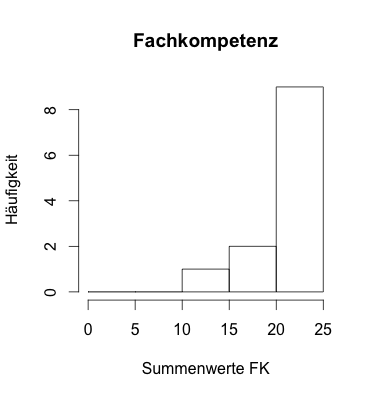
\includegraphics[width=0.33\textwidth]{Anhang/FKHist.png}
\caption{Histogramm Fachkompetenz}
\end{figure}

\begin{table}[H]
\centering
\caption{Lage- und Streumaße Fachkompetenz}
\begin{tabular}{rrrrrrrr}
  \hline
  N & Minimum & Maximum & Mittelwert & Median & Modus & SD & Varianz \\
  \hline
 12.00 & 14.00 & 25.00 & 20.58 & 21.00 & 21.00 & 3.03 & 9.17 \\
   \hline
\end{tabular}
\end{table}

\begin{itemize}
\tightlist
\item
  Methodenkompetenz Bei der Methodenkompetenz wurde der Zuwachs von
  keinem Teilnehmer auf Null, aber von drei Teilnehmer als gering
  eingeschätzt. Knapp zweidrittel der Teilnehmer (ca 59\%) schätzen
  ihren methodischen Kompetenzzuwachs auf mittel ein, etwa 17\% auf
  hoch.
\end{itemize}

\begin{table}
\centering
\caption{Häufigkeitstabelle Methodenkompetenz}
\begin{tabular}{rrrr}
  \hline
 & absolut & Prozent & kumuliert \\
  \hline
(0,5] & 0.00 & 0.00 & 0.00 \\
  (5,10] & 3.00 & 25.00 & 25.00 \\
  (10,15] & 7.00 & 58.33 & 83.33 \\
  (15,20] & 2.00 & 16.67 & 100.00 \\
  (20,25] & 0.00 & 0.00 & 100.00 \\
   \hline
\end{tabular}
\end{table}

\begin{figure}[H]
\centering
\caption{Histogramm Methodenkompetenz}
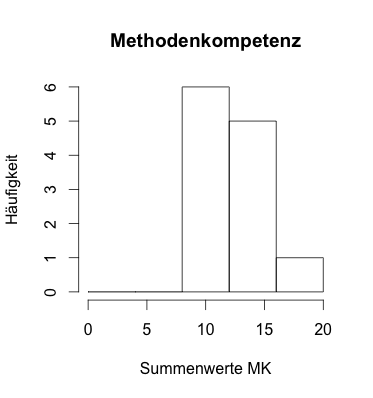
\includegraphics[width=0.33\textwidth]{Anhang/MKHist.png}
\end{figure}

\begin{table}[H]
\centering
\caption{Lage- und Streumaße Methodenkompetenz}
\begin{tabular}{rrrrrrrr}
  \hline
  N & Minimum & Maximum & Mittelwert & Median & Modus & SD & Varianz \\
  \hline
  12.00 & 10.00 & 17.00 & 12.83 & 12.50 & 10.00 & 2.41 & 5.79 \\
   \hline
\end{tabular}
\end{table}

\begin{itemize}
\tightlist
\item
  Personalkompetenz
\end{itemize}

\begin{table}[H]
\centering
\caption{Häufigkeitstabelle Personalkompetenz}
\begin{tabular}{rrrr}
  \hline
 & absolut & Prozent & kumuliert \\
  \hline
(0,5] & 0.00 & 0.00 & 0.00 \\
  (5,10] & 0.00 & 0.00 & 0.00 \\
  (10,15] & 1.00 & 8.33 & 8.33 \\
  (15,20] & 8.00 & 66.67 & 75.00 \\
  (20,25] & 3.00 & 25.00 & 100.00 \\
   \hline
\end{tabular}
\end{table}

\begin{figure}[H]
\centering
\caption{Histogramm Personalkompetenz}
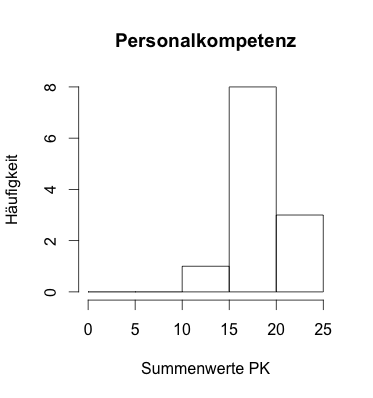
\includegraphics[width=0.33\textwidth]{Anhang/Persohist.png}
\end{figure}

\begin{table}[H]
\centering
\caption{Lage- und Streumaße: Personalkompetenz}
\begin{tabular}{rrrrrrrr}
  \hline
  N & Minimum & Maximum & Mittelwert & Median & Modus & SD & Varianz \\
  \hline
  12.00 & 11.00 & 23.00 & 19.17 & 19.00 & 19.00 & 3.04 & 9.24 \\
   \hline
\end{tabular}
\end{table}

\begin{itemize}
\tightlist
\item
  Kommunikationskompetenz
\end{itemize}

\begin{table}[H]
\centering
\caption{Häufigkeitstabelle Kommunikationskompetenz}
\begin{tabular}{rrrr}
  \hline
 & absolut & Prozent & kumuliert \\
  \hline
(0,4] & 0.00 & 0.00 & 0.00 \\
  (4,8] & 1.00 & 8.33 & 8.33 \\
  (8,12] & 5.00 & 41.67 & 50.00 \\
  (12,16] & 4.00 & 33.33 & 83.33 \\
  (16,20] & 2.00 & 16.67 & 100.00 \\
   \hline
\end{tabular}
\end{table}

\begin{figure}[H]
\centering
\caption{Histogramm Kommunikationskompetenz}
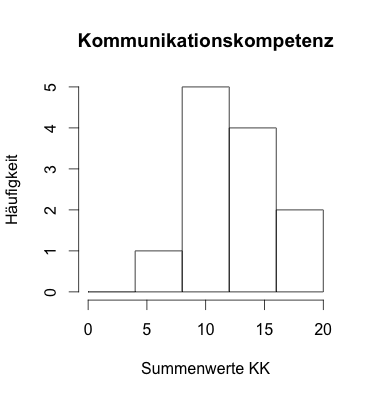
\includegraphics[width=0.33\textwidth]{Anhang/KKHist.png}
\end{figure}

\begin{table}[ht]
\centering
\begin{tabular}{rrrrrrrr}
  \hline
  N & Minimum & Maximum & Mittelwert & Median & Modus & SD & Varianz \\
  \hline
 12.00 & 8.00 & 18.00 & 13.00 & 12.50 & 9,11,16,18 & 3.54 & 12.55 \\

\end{tabular}
\end{table}

\begin{itemize}
\tightlist
\item
  Nutzungsverhalten
\end{itemize}

\begin{table}[H]
\centering
\caption{Nutzungsverhalten}
\begin{tabular}{rrrr}
  \hline
 & absolut & Prozent & kumuliert \\
  \hline
(0,10] & 1.00 & 8.33 & 8.33 \\
  (10,20] & 10.00 & 83.33 & 91.67 \\
  (20,30] & 1.00 & 8.33 & 100.00 \\
  (30,40] & 0.00 & 0.00 & 100.00 \\
   \hline
\end{tabular}
\end{table}

\begin{figure}[H]
\centering
\caption{Histogramm Nutzungsverhalten}
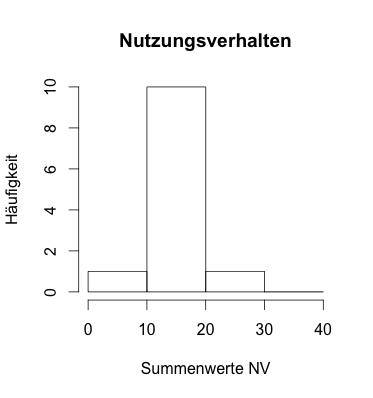
\includegraphics[width=0.33\textwidth]{Anhang/NVHist.png}
\end{figure}

\begin{table}[ht]
\centering
\begin{tabular}{rrrrrrrr}
  \hline
  N & Minimum & Maximum & Mittelwert & Median & Modus & SD & Varianz \\
  \hline
 12.00 & 9.00 & 21.00 & 16.42 & 17.50 & 14,19 & 3.32 & 10.99 \\     
   \hline
\end{tabular}
\end{table}

\begin{itemize}
\tightlist
\item
  Handlungskompetenz
\end{itemize}

\begin{table}[H]
\centering
\caption{Häufigkeitstabelle Handlungskompetenz}
\begin{tabular}{rrrr}
  \hline
 & absolut & Prozent & kumuliert \\
  \hline
(0,22.5] & 0.00 & 0.00 & 0.00 \\
  (22.5,45] & 1.00 & 8.33 & 8.33 \\
  (45,67.5] & 6.00 & 50.00 & 58.33 \\
  (67.5,90] & 5.00 & 41.67 & 100.00 \\
   \hline
\end{tabular}
\end{table}

\begin{figure}[H]
\centering
\caption{Histogramm Handlungskompetenz}
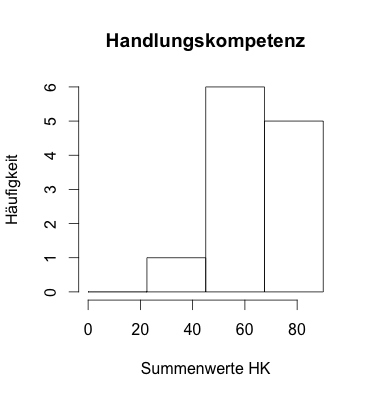
\includegraphics[width=0.33\textwidth]{Anhang/HKHist.png}
\end{figure}

\begin{table}[H]
\centering
\caption{Lage- und Streumaße der Handlungskompetenz}
\begin{tabular}{rrrrrrrr}
  \hline
  N & Minimum & Maximum & Mittelwert & Median & Modus & SD & Varianz \\
  \hline
12.00 & 44.00 & 75.00 & 65.58 & 65.50 & 63,75 & 8.49 & 72.08 \\
   \hline
\end{tabular}
\end{table}

\begin{table}[H]
\centering
\caption{Gesamtkompetenz und Nutzungsverhalten}
\begin{tabular}{rr}
  \hline
 Parameter & Mittelwerte\\
  \hline
Gesamtscore.Kompetenzen & 65.58 \\
  Mittelwert.Kompetenzen & 3.60 \\
  Gesamtscore.Nutzungsverhalten & 16.42 \\
  Mittelwert.Nutzungsverhalten & 2.05 \\
  Gesamtscore.passive.Nutzung & 10.17 \\
  Mittelwert.passive.Nutzung & 2.54 \\
  Gesamtscore.aktive.Nutzung & 6.25 \\
  Mittelwert.aktive.Nutzung & 1.56 \\
   \hline
\end{tabular}
\end{table}

\pagebreak

\pagebreak
\printbibliography
\pagebreak
\appendix


  \section{Anhang}
  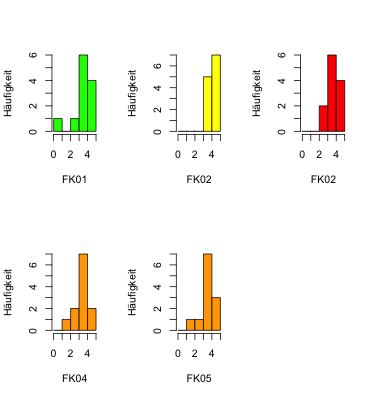
\includegraphics{Anhang/schoen.png}
  %\subsection{Abkürzungen}
  %\renewcommand{\thetable}{{A}.\arabic{table}}
  %\renewcommand{\thetable}{\Alph{section}.\arabic{table}}
  \begin{table}[H]
\centering
%\captionof{table}[Anhang]{Titel}
%\caption{Zuordnung der Items}
\label{itemtabelle}
\resizebox{\textwidth}{!}{%
\begin{tabular}{@{}lllll@{}}
\toprule
Item  & Konstrukt                                                                    & Indikator                                                                                                                                                                           & Ausprägung                                                                                                                                                                                       & Skalenniveau \\ \midrule
1-5   & \begin{tabular}[c]{@{}l@{}}Fach-\\ kompetenz\\FK1,FK2,FK3,FK4,FK5\end{tabular}                    & \begin{tabular}[c]{@{}l@{}}Disposition sachlich-gegenständliche\\ Probleme selbstorganisiert lösen zu können\end{tabular}                                                           & \begin{tabular}[c]{@{}l@{}}5-stufige Likertskala:\\ 1= trifft überhaupt nicht zu\\ 2= trifft wenig zu\\ 3=trifft teils/teils zu\\ 4=trifft überwiegend zu\\ 5=trifft völlig zu\end{tabular}      & metrisch     \\
\midrule
6-10  & \begin{tabular}[c]{@{}l@{}}Methoden-\\ kompetenz\\MK1,MK2,MK3,MK4\end{tabular}                & \begin{tabular}[c]{@{}l@{}}Tätigkeiten und Aufgaben methodisch\\  selbst-organisiert zu gestalten und Methoden\\  weiter zu entwickeln\end{tabular}                                 & \begin{tabular}[c]{@{}l@{}}5-stufige Likertskala: \\ 1= trifft überhaupt nicht zu\\ 2= trifft wenig zu \\ 3=trifft teils/teils zu \\ 4=trifft überwiegend zu \\ 5=trifft völlig zu\end{tabular}  & metrisch     \\
\midrule
11-16 & \begin{tabular}[c]{@{}l@{}}Personal-\\ kompetenz\\PK1,PK2,PK3,PK4,PK5\end{tabular}                & \begin{tabular}[c]{@{}l@{}}Sich einschätzen, selbstorganisiert reflexiv\\  handeln,Werte, Motive und Selbstbilder\\  entwickeln\end{tabular}                                        & \begin{tabular}[c]{@{}l@{}}5-stufige Likertskala: \\ 1= trifft überhaupt nicht zu \\ 2= trifft wenig zu \\ 3=trifft teils/teils zu \\ 4=trifft überwiegend zu \\ 5=trifft völlig zu\end{tabular} & metrisch     \\
\midrule
17-21 & \begin{tabular}[c]{@{}l@{}}Komunikations-\\ kompetenz\\KK1,KK2,KK3,KK4\end{tabular}           & \begin{tabular}[c]{@{}l@{}}Sich mit anderen kreativ auseinander setzen, \\ kommunikativ und selbstorganisiert handeln\\ \parencite[8]{ErpenbeckRosenstiel200305}\end{tabular} & \begin{tabular}[c]{@{}l@{}}5-stufige Likertskala\\ 1= trifft nicht zu,\\2= trifft wenig zu \\ 3=trifft teils/teils zu \\ 4=trifft überwiegend zu \\ 5=trifft vollständig zu\end{tabular}                                                                                    & metrisch     \\
 \midrule
22-28 & \begin{tabular}[c]{@{}l@{}}Nutzungs\\ verhalten\\ Lernplattform NV1,NV2,NV3\\NV4,NV5,NV6,NV7,NV8\end{tabular} & \begin{tabular}[c]{@{}l@{}}Aufschluss über die Intensität u\\ der Nutzung der Lernplattform\end{tabular}                                                                 & \begin{tabular}[c]{@{}l@{}}5-stufige Skala\\ 1=0-1mal genutzt\\ 2=2-4 mal genutzt\\ 3=5-7 mal genutzt\\ 4=8-10 mal genutzt\\ 5=\textgreater10 mal genutzt\end{tabular}                            & metrisch     \\ \bottomrule
\end{tabular}%
}
\end{table}



%\input{tabelleanalysen}
%\includepdf{alleine.pdf}
\end{document}
